\documentclass[11pt]{article}
\usepackage[margin=1.1in]{geometry}
\usepackage{amsmath,amssymb}
\usepackage{mathpazo}
\usepackage[T1]{fontenc}
\usepackage{microtype}
\usepackage[hidelinks]{hyperref}
\usepackage{graphicx}
\usepackage{parskip}
\setlength{\parskip}{6pt}
\usepackage{titlesec}
\titleformat{\section}{\large\bfseries}{\thesection.}{0.6em}{}
\titleformat{\subsection}{\normalsize\bfseries}{}{0em}{}
\begin{document}



\begin{center}{\LARGE\bfseries Motion-Only Capsize Warning on an Audited Synthetic Benchmark: Ranking Skill Without Threshold Transfer}\end{center}

\textbf{W. R. Story}

\section*{Abstract}

Can the measured roll motion of a ship warn of capsize soon enough to act, at a false-alarm
cost a crew could accept? We study this question on a synthetic benchmark validated against
analytic limits and internal numerical checks; external ship-level validity is out of scope: a
one-degree-of-freedom nonlinear roll model, three restoring-curve families representing
distinct ways a ship loses stability, and 58,500 seeded trajectories under JONSWAP forcing.
Five warning methods compete under one protocol in which every operating threshold is chosen on
calibration data and frozen before each test evaluation, with every historical deviation from
that protocol recorded in the repository rather than repaired silently: a small convolutional
network, classical variance
and autocorrelation trend statistics, a likelihood-ratio detector, a closed-form
critical-roll-rate margin, and a phase-space neighbor-count score. Four findings emerge.
(a) Ranking skill is real at every forcing bandwidth tested; the fixed-window primary network
separates dangerous from ordinary intervals with window AUC 0.883 to 0.913. (b) Inside an
established severe regime, no tested motion-only statistic predicts which encounter will be fatal;
all score near chance. (c) Most nominally
false alarms, 75 to 88 percent, coincide with high-envelope wave-group episodes, a coincidence
proxy without a matched null, that the vessel survived. (d) No method's threshold transfers across failure modes at fixed sensitivity. We
then operate the split-time upcrossing decomposition as an onboard rate estimator, in online
and offline-calibrated forms; both fail preregistered calibration tests for a reason we
localize. In an in-sample check, the decomposition reproduced realized counts: given the
empirically measured probability that a
threshold crossing is terminal, it reproduces realized counts within 3 in 71. But the
closed-form criticality model overestimates the lethality of a crossing by roughly a factor of
four, and in 92 percent of capsizes the crossing that matters arrives less than ten seconds
before the event. An audit during the study found our own first results inflated by test-set
threshold selection; every number reported here is the corrected value. The picture that
survives is simple, and a final embedded-group experiment quantifies it within its own design.
Embedding a frozen library of six wave-group shapes at six prescribed heights into independent
irregular preludes, so that the vessel arrives at each group naturally, capsize within the
group is predicted at AUC 0.513 from the vessel's entry state, 0.934 from the group's
engineered descriptors, and 0.938 from both. Within that balanced single-configuration
experiment, motion reveals the slowly building vulnerability and the arriving group's
description dominates the rest.

\emph{Highlights:} five motion-only capsize detectors under a preregistered, audited protocol;
ranking skill survives every forcing bandwidth, but alarm thresholds do not transfer; within an
established severe regime, every motion statistic times capsize at chance; the split-time
decomposition, operated online for the first time, miscalibrates by a factor of four; in a
balanced embedded-group experiment, group descriptors reach AUC 0.93 while entry state adds 0.004.

\emph{Keywords:} capsize, intact stability, real-time warning, split-time method, preregistered
evaluation, synthetic benchmark.

\section{Introduction}

Begin from first principles. A ship in beam seas is a lightly damped nonlinear oscillator:
waves push, the righting arm restores, and capsize is the escape of that oscillator over the
rim of its potential well. Two different questions hide inside ``can we warn?'' One asks whether
the well is becoming shallow --- vulnerability, a slow process. The other asks when a particular
group of waves will push the ship over --- the encounter, a fast one. Every result in this paper
answers one of those two questions, and the paper's central finding is that motion measurement
answers only the first.

Interest in warning of capsize from onboard motion measurement is at least two decades old. The
Lyapunov-exponent programme of the mid-2000s (McCue and Troesch 2004, 2006) sought a precursor
of capsize in the divergence of measured trajectories; the author's
thesis in that programme (Story 2009) found empirically that the useful signal lay not in
estimated exponents but in the loss of phase-space neighbors, and reported a neighbor-count
warning flag with encouraging lead times and an honestly documented false-alarm problem. The
thread was not taken up. The signal-based detectors of Galeazzi et al. (2013, 2015) for
parametric roll, with designed false-alarm probabilities and full-scale blind validation, remain
the only fielded success of motion-based stability-failure detection, and the field's general
machinery moved instead to offline probabilistic assessment (Belenky and Sevastianov 2007), of
which the split-time method (Belenky, Weems and Lin 2016; Belenky et al. 2024) is the principal
example, and to operational guidance derived from precomputed simulation under the
second-generation intact stability criteria (Ba\v{c}kalov et al. 2016; IMO 2020; Petacco and Gualeni
2020; Shigunov 2023).

The relationship of the present work to the split-time method deserves statement at the outset,
since that method supplies both the strongest available machinery and the sharpest open question.
Belenky et al. (2024) compute the probability of capsizing offline. Their central object is an
upcrossing: the roll angle passing outward through a fixed intermediate threshold, here the
angle of maximum righting arm. The metric of danger, a critical roll rate at those upcrossings,
is evaluated along simulated histories, its tail is
extrapolated with a physics-informed exponential form (Glotzer et al. 2024), and the estimate
is validated by confidence-interval capture against direct counting (Weems et al. 2023; on
direct-counting interval estimands see Wandji et al. 2024). Three transfers from that programme are
attempted here. The metric itself is operated, to our knowledge for the first time, as a
continuously evaluated onboard alarm statistic computed from measured state alone, and is
benchmarked against learned and statistical competitors on equal terms. The statistical
discipline of the split-time programme, declustering, interval estimates on every rate, and
validation against direct counting, is transplanted to warning evaluation, where it is presently
absent. And the boundary of the transfer is itself measured: the engineering-fidelity form of the
metric requires re-simulation with the incident wave realization known, and the present results
quantify operationally what that requirement conceals, namely that the information carried by the
future waves is absent from measured motion precisely where event timing is decided.

The present study returns to the motion-only question with tools that did not exist in 2009 and
with an evaluation protocol designed against the failure modes that make warning research easy to
overstate. A warning method may rank dangerous intervals well yet possess no usable threshold; a
threshold may fail to transfer across failure modes or sea states; apparent skill may arise from
protocol time, truncated outcome windows, or the use of future data during normalization; and,
because capsizes are rare, an aggregate score conceals all of these. Each failure mode is tested
separately here. The study also reports, deliberately, an audit of its own methodology: the
operating points first obtained were later found to have been selected on test outcomes, an error
we believe is widespread in the published literature on learned motion prediction, and
the corrected results quantify its size.

Three questions are addressed. First, does motion history rank capsize risk under forcing broad
enough that classical critical-slowing-down indicators fail? Second, do the resulting operating
thresholds transfer across stability-failure modes at fixed sensitivity? Third, what do the false
alarms of such systems consist of?

\section{The synthetic benchmark}

The benchmark is the simplest ship that can capsize (Figure 1): a one-degree-of-freedom
nonlinear roll model, validated against analytic limits, generating seeded trajectories under
JONSWAP forcing (Hasselmann et al. 1973). Three restoring
families represent failure archetypes: softening restoring (dead-ship escape), time-varying
stiffness (parametric roll), and biased restoring with asymmetric escape angles (damage, steady
heel), in the scope of established one-degree-of-freedom roll comparisons (Bulian and
Francescutto 2004, 2011). Following-sea failure modes, broaching foremost (Umeda et al. 2016),
are outside the benchmark's scope, a limitation the transfer results of Section 5 should be read
against. Forcing is synthesized spectrally with deterministic amplitudes and
seeded random phases (Shinozuka and Deodatis 1991); integration is fixed-step Runge-Kutta at no
fewer than 40 steps per natural period; capsize is an absorbing state and post-event samples are
excluded from every window.

Validation gates precede all warning experiments: recovered significant wave height within 2
percent; linear-limit response variance within 6 percent of the spectral calculation; the
principal Mathieu boundary within 10 percent of the averaging result; and the simulated harmonic
capsize boundary at or above the heteroclinic Melnikov threshold (Falzarano, Shaw and Troesch
1992) with the correct frequency shape, the bound being treated as a necessary condition only. No
validation test is skipped in the acceptance run.

The reference data comprise 58,500 trajectories of 600 seconds at a four-second natural period:
stationary campaigns per family, stiffness-ramp campaigns representing slow stability erosion,
one sea-state step campaign, rare-event evaluation campaigns at 0.95 to 2.0 percent capsize
rates, and five forcing-bandwidth campaigns in which JONSWAP peak enhancement is varied from 1.0
to 30 with terminal ramp severity retuned per bandwidth so that outcome rates remain in a common
band; the last decision prevents severity from acting as a hidden bandwidth axis. Disjoint seed
blocks separate training, calibration, test, and guarded holdout data.

Supervised windows use 60 natural periods of causally normalized roll and roll-rate history, a
50-period outcome horizon, and an exclusion band for near misses; a future-only leakage probe
verifies the entire feature path against a deliberately leaky control. The label discipline
responds directly to critiques of early-warning-signal studies in other fields (Boettiger and
Hastings 2012; Dakos et al. 2012).

\begin{figure}[t]\centering\includegraphics[width=\linewidth]{figs/fig_model.png}\caption{The benchmark. (a) The three restoring families: the softening curve with its escape angles (dashed red), the constant bias moment that shifts the biased family's equilibria, and the parametric family's stiffness modulation envelope (dotted). (b) Two 600-second lives of the same ship in the same sea state, different seeded seas: the capsizing life ends during a wave group in its first minute, while its twin survives larger excursions for the full record. The encounter, not the general severity, decides the moment.}\end{figure}

\section{Five warning methods}

All five methods consume identical windows and emit a scalar score which is thresholded into
alarm episodes (three consecutive crossings to open; refractory closure). No method receives wave
elevation, spectrum, family identity, or sea-state input.

(a) A temporal convolutional network of 2,969 parameters trained on the horizon labels, in the
spirit of learned early-warning classifiers (Bury et al. 2021); neural roll prediction has
in-community precedent (M\'iguez Gonz\'alez et al. 2023). (b) Rolling variance and lag-one
autocorrelation with Kendall trend statistics, the classical critical-slowing-down indicators
(Dakos et al. 2012), whose rate-of-change and noise-model limits are themselves documented
(Radhakrishnan et al. 2025; Layritz et al. 2025). (c) A roll-power adaptation of the double-Weibull generalized
likelihood-ratio detector of Galeazzi et al. (2013, 2015). (d) The split-time critical
roll rate (Belenky et al. 2024), computed in closed form from the known restoring parameters and
the measured state, with the separatrix line extrapolated between threshold crossings; to our
knowledge this quantity has not previously been operated as a continuously evaluated
online alarm statistic, and it functions here as a zero-training physics baseline. (e) The
neighbor-count score of Story (2009), reimplemented faithfully in the (roll, roll-rate) plane
under strictly causal normalization, with the thesis's fixed flag retained as one point on a full
operating curve; phase-space identification of dangerous ship states has since been developed
independently in the Spyrou school (Kontolefas and Spyrou 2020).

\section{Evaluation protocol and the audit}

Metrics are episode sensitivity, false episodes per exposure hour, and lead time, with
trajectory-block bootstrap intervals and fixed campaign weights; exposure ends at capsize; an
episode overlapping the pre-capsize horizon is event-associated. All operating controls are
selected on calibration data, frozen, and evaluated once on test data.

The protocol was not followed from the outset, and the failure is reported as a result. The
study's first operating points were obtained by scanning test-set metrics for the lowest
false-episode rate at 90 percent sensitivity or better, which is threshold selection on test
outcomes. Reported false-episode rates under test-informed selection were several times lower
than the calibration-frozen rates reported after correction; because the affected evaluations
differ in population as well as threshold provenance, we report the effect qualitatively rather
than as a single controlled factor. One guarded holdout evaluation was additionally invalidated
by threshold selection on the holdout labels, and its artifacts are retained as historical
records only. The corrected protocol is enforced by the test suite rather than by convention.
We suggest that reported operating points in the learned motion-prediction literature should be
read with this mechanism in mind wherever threshold provenance is not stated.

\section{Results}

\textbf{Ranking under bandwidth (D3).} The fixed-window primary network's window AUC was 0.883 to
0.913 at every peak enhancement from 30 down to 1.0, while the classical trend indicators collapsed on ramped
campaigns. Ranking skill from motion history survives broadband forcing. The predeclared
operating-cost criterion at the broadband end (a 10 percent false-episode improvement) was missed
at 7.6 percent (14.061442 versus 15.212539 false episodes per hour), and the operating-cost claim
is reported as inconclusive: ranking skill and a deployable threshold are different assets
(Figure 2).

\begin{figure}[t]\centering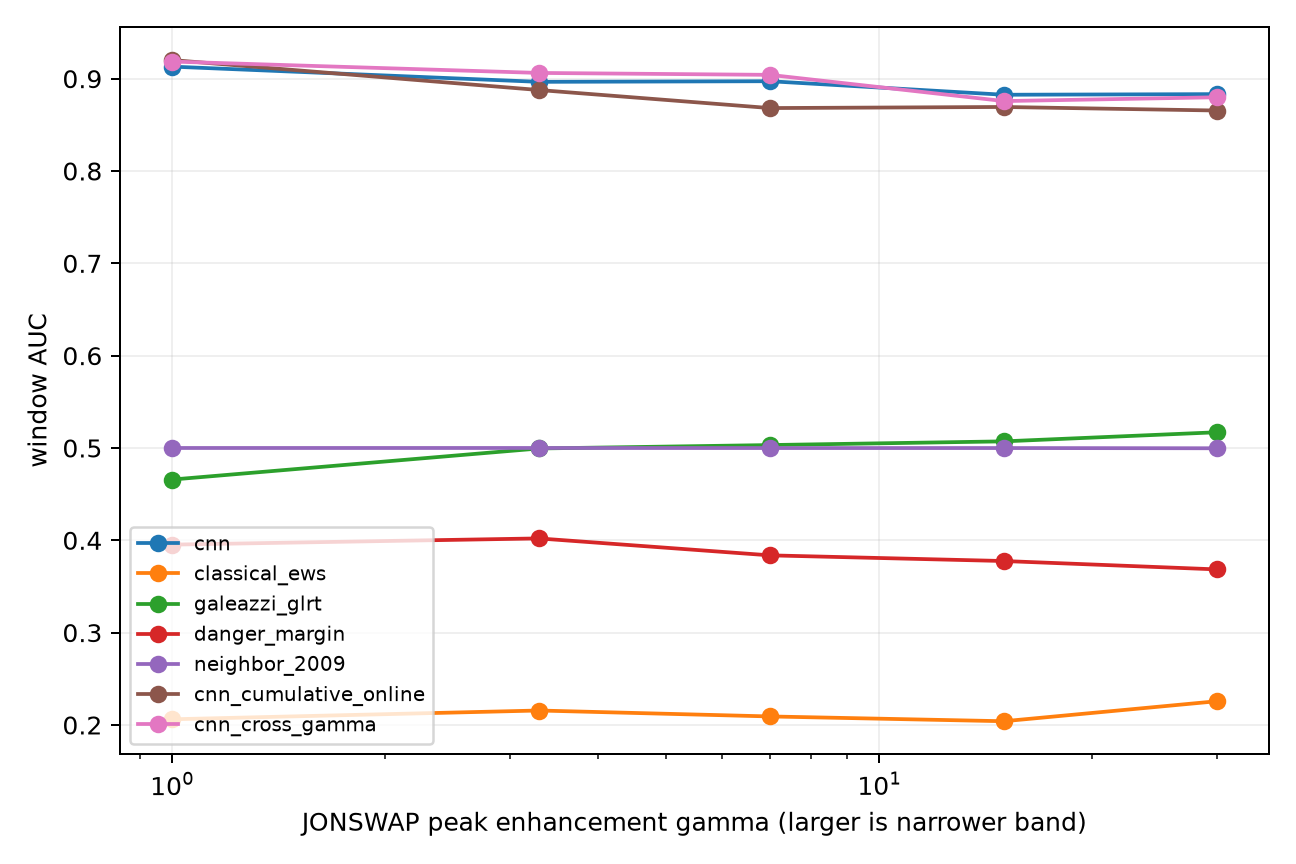
\includegraphics[width=\linewidth]{../../results/d3_bandwidth_skill_v02.png}\caption{Ranking survives bandwidth. Window AUC on the five forcing-bandwidth campaigns, corrected record: the fixed-window primary network holds 0.883 to 0.913 from narrow-band forcing down to fully broadband, while the classical indicators and physics scores range from near chance to well below it on these ramped campaigns --- the fixed-window scoring that is honest about information also strips the trends those baselines rely on.}\end{figure}

\textbf{Pooled operating points (D1).} At calibration-frozen thresholds on the pooled rare-event
campaigns, the fixed-window primary network attained 91.00 percent sensitivity at 13.409 false
episodes per hour; the classical indicators reached 100 percent sensitivity only at a
near-always-on threshold costing
21.4 per hour; the physics margin and the 2009 neighbor score occupied the same
high-sensitivity, high-cost region. No method reached 90 percent sensitivity at a false-episode
rate below several per hour (Figure 3).

\begin{figure}[t]\centering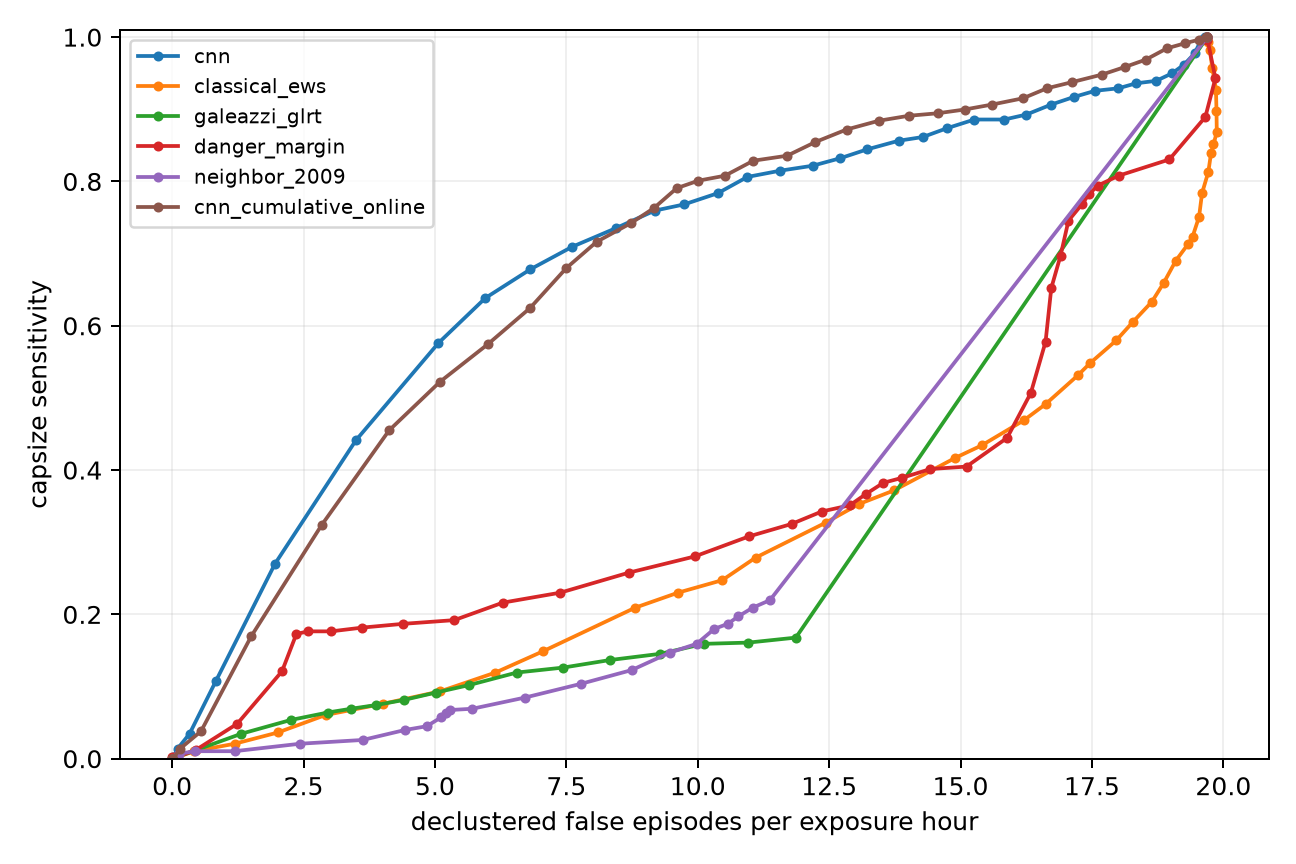
\includegraphics[width=\linewidth]{../../results/d1_operating_curves_v02.png}\caption{The pooled operating curves, corrected record: capsize sensitivity against declustered false episodes per exposure hour at calibration-frozen thresholds. The network variants dominate the low-cost region; every classical and physics score buys sensitivity only near the always-on corner. Even the best curve pays several false episodes per hour at 90 percent sensitivity.}\end{figure}

\textbf{Threshold transfer (D2).} The fixed-window CNN reached 99.15 percent, 90.83 percent, and
76.21 percent test sensitivity across the softening, parametric, and biased holdouts. Two
rotations met 90 percent, but only near always-on alarm cost; the biased holdout failed. No
deployable transfer was established.

\textbf{Within-regime discrimination (D5).} After the full wash-in, the fixed-window CNN's
orientation-independent AUC was 0.556, below the 0.58 trigger; cumulative-online CNN reached
0.538 and classical scores remained near chance. Motion-only scores carried no usable information
about which encounter would be terminal inside the established severe regime.

\textbf{Finite-time tangent result (F1).} The non-tangent level, rate, energy, and strain statistics
remain scoped to their stated full F1a estimand. Conditional on windows whose trajectories
survived through each tested finite-time tangent horizon, no finite-time tangent statistic
exceeded chance. The latter is a descriptive result for the tested statistic family, not an
information-theoretic bound; the labels-only censoring counts are recorded in the dated addendum.

\textbf{The character of false alarms (D4).} Between 75 and 88 percent of nominally false episodes
coincided with high-envelope wave groups, defined by an envelope criterion on the known
synthetic seaway, that the vessel survived. This is a coincidence proxy, not the
critical-wave-groups method proper (Themelis and Spyrou 2007; Anastopoulos et al. 2016). The
pooled range also mixes artifact generations: the danger-margin row is v0.2-regenerated while
the remaining rows are v0.1-corrected, as the repository's supersession tables record. The
figure is descriptive, since no matched null was
tested and groups are common in a narrow-band sea; its qualitative content is that outcome-based
false-positive accounting charges the detectors for hazard exposure the vessel happened to
survive, the base-rate structure anticipated in Boettiger and Hastings (2012).

\textbf{Reference comparators.} On the v0.2 design-balanced window set, the exact-state independent-
future restart reached AUC 0.850, fixed-window XGBoost 0.723, and fixed-window CNN 0.652; a
protocol-time comparator also exceeded the network. Two qualifications apply: the restart
comparators replace the realized forcing and are therefore reference points rather than bounds,
since the temporally correlated seaway leaves encounter information in the motion history; and
part of the network's advantage on natural test populations evidently derived from population
structure rather than state inference. The headroom that exists lies in state inference, and
simple tools claimed it first.

\textbf{The split-time rate estimator (U1, H1).} Three preregistered experiments operated the
paper's ROM decomposition --- capsize rate as upcrossing rate times the probability an upcrossing
goes critical --- as a continuously updated onboard estimate, each evaluated once on fresh test
data by the split-time program's own confidence-interval-capture standard. The
online-estimated form failed its capture criterion, and a predeclared comparison found the
upcrossing rate alone more reliable than the full decomposition, so the corresponding kill
criterion fired. A measured attribution then localized the error: with the empirical
terminal-crossing probability substituted for the modeled one, the decomposition predicted 68
events against 71 realized, while the closed-form criticality model (the unforced
piecewise-linear critical roll rate with an exponential tail) overpredicted by roughly a factor
of four; a motion-derived estimate of the forced correction made the error larger, not smaller.
A final hybrid, with the conditional calibrated offline from design-stage data and multiplied
onboard by the measured crossing rate, also failed its capture and transfer criteria. A timing
audit supplied the mechanism: in 92 percent of heralded capsizes (19 exceptions in 240) no
emission interval separated the terminal crossing from the capsize, so the severity information
the conditional carries becomes available only after the event has begun. Two methodological
qualifications attach: fresh test slices of 30 to 60 expected events realized counts 21 to 37
percent from expectation, and the capture intervals carried parameter uncertainty without
realization noise, so the capture criterion on slices of this size is severe even for a
correctly calibrated estimator; the reliability errors (0.039848 for the hybrid, 0.042806 for the
rate-only map, and 0.242303 for a variance-based map) are the fairer calibration comparison. All
verdicts were preregistered and stand as recorded. Figure 4's middle panel shows the one
encouraging pattern: the crossing rate alone, offline-mapped, tracks the reliability diagonal
more closely than either alternative, though every method failed the count-capture criterion.

\begin{figure}[t]\centering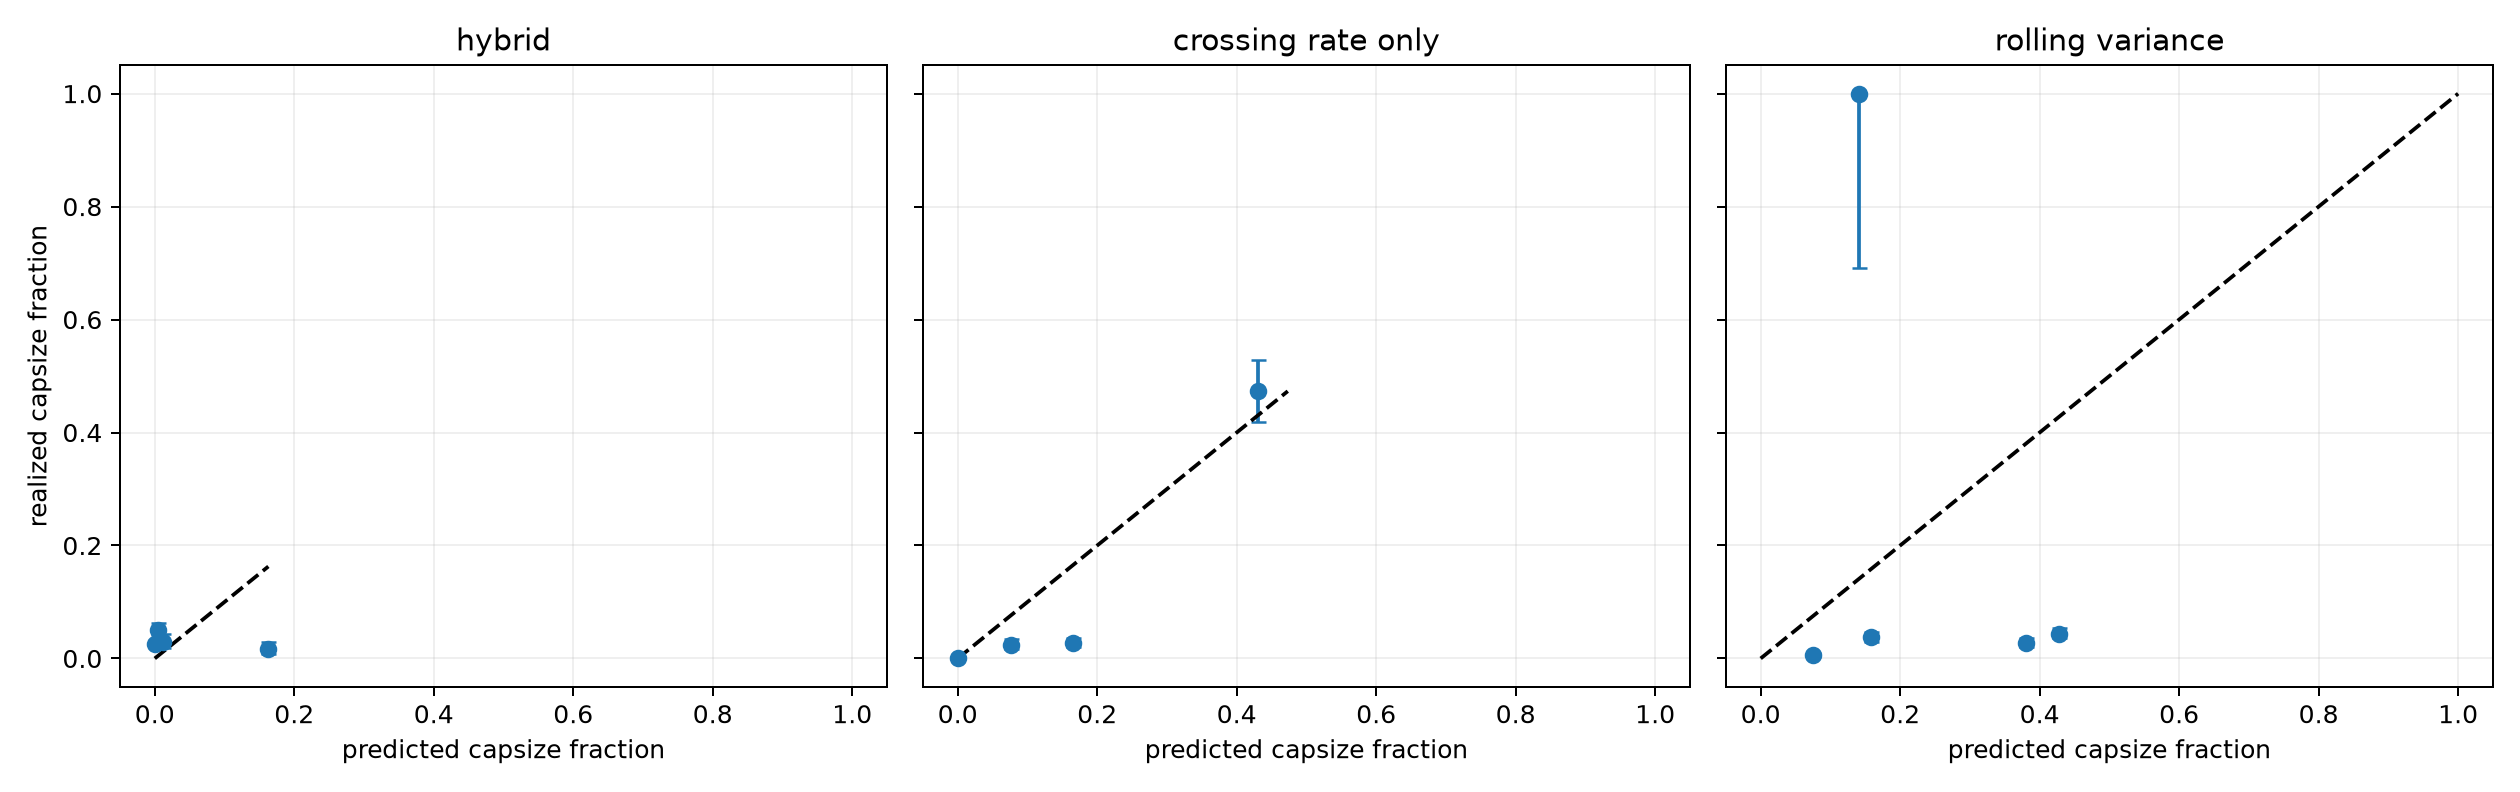
\includegraphics[width=\linewidth]{../../results/h1_reliability_h1.png}\caption{Reliability of the offline-calibrated hybrid and its comparators on fresh test data (H1): predicted capsize probability per bin against the realized fraction. The hybrid under-predicts throughout; the crossing-rate-only map tracks the diagonal; the variance map scatters. The observable factor of the split-time decomposition --- the crossing rate --- carries the calibration.}\end{figure}

\textbf{The exponent's clean trial (F1).} The 2009 thread deserved one experiment its era could not
run: the finite-time Lyapunov exponent computed exactly, from the model's analytic Jacobian,
with tangent perturbations receiving the identical realized forcing (the standard construction
of Babaee et al. 2017). One preregistered ablation evaluated the margin level, its closure
rate, time to closure, energy reserve and depletion, level-plus-rate combinations, the
instantaneous strain normal to the escape boundary, and generic and escape-directed finite-time
exponents, in both an operational causal setting and an oracle setting with the true state and
tangent map. On the fully post-step severe-regime geometry, every statistic scored between
0.501 and 0.507 --- including the acausal true-tangent exponents, which use information from the
future itself. The conditional plan to audit the 2009 estimator's implementation was therefore
retired by its own trigger: within this tested family of statistics, the exactly computed
quantity itself carried no timing information, so any historical implementation defect was
immaterial to the thesis's conclusion. Two scope notes apply: finite-time scores are evaluated
on windows whose trajectory survives the tangent horizon (in-horizon capsizes are censored, a
population the addendum quantifies), and the escape-directed score is a custom projection onto
the initial-state escape normal, not the conventional singular-value exponent (Shadden et al.
2005). The thesis's empirical pivot away from
exponents was correct at the level of the underlying quantity.

\textbf{The other side of the decomposition (D4b).} A final experiment asked the question every
negative above implies: if the arriving wave group were known, how much would it decide? A
frozen library of six envelope-mined group shapes was embedded into hundreds of independent
irregular preludes, in the natural-initial-condition manner of Silva and Maki (2021, 2024;
extended to free-running vessels in Silva and Maki 2026), so that
the vessel and its response history arrive at each group naturally; group heights were swept
across the critical range and monotone response maps fitted per entry-state stratum. Evaluated
once on held-out preludes (7,164 trials, 580 capsizes), capsize within the group was predicted
at AUC 0.513 [0.503, 0.524] from the vessel's entry state alone --- chance --- at 0.934
[0.930, 0.938] from the group's engineered descriptors alone, and at 0.938 [0.934, 0.941] from
both, with intervals from prelude-level bootstrap resampling. The preregistered expectation
that the combination would substantially exceed either input was honestly not confirmed: the
entry state adds 0.004 of AUC once the group is known. The estimand deserves precision: this is
a balanced design over six frozen shapes and six prescribed heights, in-support (shapes and
heights are not held out; prelude seeds are), for one softening-family configuration in beam
seas, and the group descriptors include the imposed height --- the experimentally manipulated
driver. Within that design, group descriptors dominate the entry state; no universal division
of predictability follows. A companion
rate composition over the library's naturally occurring groups failed its capture criterion in
the informative direction --- every library class fell below its critical height, so real
capsizes arise from sequences beyond the mined classes. This six-class implementation failed
coverage of the direct capsize mechanism; no conclusion about other libraries or
parameterizations follows, and broadband group representations with initial-condition
variability (Hafezi et al. 2026; cf. Anastopoulos and Spyrou 2019, 2023) indicate what a
broader library must include. A preregistered wave-field audit preceded these runs: the periodic record's
recurrence begins beyond every labeled lag; elevation upcrossing rates match the Rice formula
in a passing-rate sense, though one preregistered continuous-Rice mean gate failed as a
consequence of the fixed-energy conditioning; and that conditioning of the
deterministic-amplitude ensemble is stated as part of the estimand.

A companion study of conformalized forecast intervals on the same benchmark (following Romano,
Patterson and Cand\`es 2019; Gibbs and Cand\`es 2021; sequential and nonexchangeable variants in
Zaffran et al. 2022, Xu and Xie 2023, and Barber et al. 2023) found stationary marginal coverage accurate to
0.75 percentage points in the mean, while every online adaptation scheme tested failed a
predeclared joint rolling-coverage and alarm-cost criterion through the sea-state step. Those
results are reported in the project record and not further discussed here.

\section{Discussion}

The results organize into a two-clock description. The slowly varying stability state, the
eroding restoring that determines whether the vessel is in danger, is observable from motion
history: ranking skill survives every forcing bandwidth, and the most informative engineered
feature is in effect an online stiffness estimate, a quantity this community has long extracted
from the roll period (Terada et al. 2016; M\'iguez Gonz\'alez et al. 2017). For the tested family of
motion-only statistics, the terminal encounter, the particular wave group that converts
vulnerability into capsize, was not recovered once the severe regime was established; the
within-regime result is chance-level for learned, classical, and physical scores alike, consistent
with the stochastic-Melnikov view that a deterministic separatrix loses its predictive meaning
under random forcing (Frey and Simiu 1993). The practical reading is that motion-only systems should be understood, and
evaluated, as vulnerability monitors rather than event predictors, a role compatible with the
operational measures framework of the second-generation criteria (IMO 2020) rather than with an
alarm bell.

Read against the split-time programme, the results locate both the value and the limit of
operating its metric onboard. As a zero-training detector the closed-form critical roll rate was
sensitivity-dominant and cost-competitive with every learned alternative, which is at once a
tribute to the physics and a caution against claims for learned detectors that have not faced it
as a baseline. Its one systematic failure, degradation on stability-erosion campaigns where the
assumed restoring becomes stale, identifies the missing component for operational use: online
estimation of the current restoring state, whose feasibility the comparator results demonstrate,
the roll period alone recovering most of the available headroom. The within-regime chance result
then explains why the engineering-fidelity metric must re-simulate with the waves known: the
future-dependent quantity used by the motion perturbation method was not recovered by the tested
motion-only statistics. The U1 and H1 experiments made that boundary quantitative from
inside the method itself. The rate factor of the decomposition, an observable of the slowly
varying stability state, survives as a usable vulnerability measure; the severity factor, which
would time the event, is in 92 percent of capsizes not emitted until the event has begun. The
two-clock description of Section 6 is therefore not an external criticism of the split-time
programme but a property its own decomposition exhibits when operated online: the rate factor
works, while the tested online severity factor requires future re-simulation.

The false-alarm finding bears on how such monitors should be judged. If three quarters or more of
false episodes are honest responses to genuine hazard exposure, then false episodes per hour,
computed against outcomes, systematically understates the value of the warning and overstates the
cost. Metrics conditioned on hazard exposure, and alarm policies whose budgets are conditioned on
regime, appear to us a more productive direction than further detector refinement.

Finally, the audit deserves a place in the discussion rather than an apology. The evaluation
stack that produced the leaked operating points had predeclared kill criteria, confidence
intervals on every rate, frozen data splits, and guarded holdouts, and it still admitted a factor
of 2.5 of optimism through threshold provenance. The mechanism is not exotic and is not confined
to this study. The community's evaluation practice for learned warning methods would benefit from
treating threshold provenance as a reportable property of every operating point.

\section{Conclusions}

On a synthetic benchmark validated against analytic limits and internal numerical checks,
spanning three stability-failure archetypes, motion-only warning methods rank capsize risk well
above chance at every forcing bandwidth tested, fail to
transfer operating thresholds across failure modes, and discriminate event timing at chance
inside an established severe regime; the majority of their false alarms coincide with
high-envelope wave-group episodes. A test-selected evaluation had earlier made the leading detector
appear two and one half times cheaper in false alarms than it is. The split-time experiments
sharpen the same conclusion from inside the method: the upcrossing rate survives as a simple,
usable vulnerability measure, while the severity term that would time the event arrives, in 92
percent of capsizes, after the event has begun. The natural-initial-condition experiment then
argues the same point from the other side: within its balanced single-configuration design,
with the arriving group's engineered description fully known, capsize within the group is
predicted at AUC 0.934 while the vessel's entry state adds 0.004. That motivates, but does not
price, a forward-sensing experiment: what was tested is a complete, noiseless, exactly aligned
episode representation, and whether any realizable sensor recovers a useful fraction of it ---
under range limits, directional ambiguity, and estimation error (Nielsen et al. 2024; Lee and
Kim 2025) --- is the proposed next study. Further progress on the timing
question appears to require information about the incident wave field rather than refinement of
motion-only architectures; shipboard sea-state and wave-field estimation is an active
literature (Nielsen 2017; Nielsen et al. 2024; Lopac et al. 2026), and the benchmark's frozen
splits and audited protocol provide the evaluation discipline for that study, though an
encounter-sensing experiment would require model extensions the benchmark does not yet
contain.

\section*{Declarations}

\textbf{Data availability.} The benchmark code, campaign definitions, preregistrations, and the
complete numerical record, including corrected and superseded results retained as immutable
history, will be public at github.com/wrobstory/rahola on publication.

\textbf{Declaration of competing interest.} The author declares no competing financial interests or
personal relationships that could have influenced this work.

\textbf{CRediT author statement.} W. R. Story: conceptualization, methodology, software,
validation, formal analysis, investigation, data curation, writing, visualization.

\textbf{Funding.} This research received no external funding.

\section*{Acknowledgments}

The benchmark code, campaign definitions, and the complete numerical record, including the
pre-audit results retained as historical artifacts, are available from the author.

\section*{References}



\hangindent=1.5em\hangafter=1\noindent Anastopoulos, P. A., and Spyrou, K. J. (2019). Evaluation of the critical wave groups method in calculating the probability of ship capsize in beam seas. \emph{Ocean Engineering} 187, 106213.\par
\hangindent=1.5em\hangafter=1\noindent Anastopoulos, P. A., and Spyrou, K. J. (2023). Extrapolation of ship capsize probability over significant wave height: foundation on wave groups theory. \emph{Ocean Engineering} 281, 114766.\par
\hangindent=1.5em\hangafter=1\noindent Anastopoulos, P. A., Spyrou, K. J., Bassler, C. C., and Belenky, V. (2016). Towards an improved critical wave groups method for the probabilistic assessment of large ship motions in irregular seas. \emph{Probabilistic Engineering Mechanics} 44, 18--27.\par
\hangindent=1.5em\hangafter=1\noindent Babaee, H., Farazmand, M., Haller, G., and Sapsis, T. P. (2017). Reduced-order description of transient instabilities and computation of finite-time Lyapunov exponents. \emph{Chaos} 27, 063103.\par
\hangindent=1.5em\hangafter=1\noindent Barber, R. F., Cand\`es, E. J., Ramdas, A., and Tibshirani, R. J. (2023). Conformal prediction beyond exchangeability. \emph{Annals of Statistics} 51(2), 816--845.\par
\hangindent=1.5em\hangafter=1\noindent Ba\v{c}kalov, I., Bulian, G., Ros\'en, A., Shigunov, V., and Themelis, N. (2016). Improvement of ship stability and safety in intact condition through operational measures: challenges and opportunities. \emph{Ocean Engineering} 120, 353--361.\par
\hangindent=1.5em\hangafter=1\noindent Belenky, V. L., and Sevastianov, N. B. (2007). \emph{Stability and Safety of Ships: Risk of Capsizing}, 2nd ed. SNAME, Jersey City.\par
\hangindent=1.5em\hangafter=1\noindent Belenky, V., Weems, K. M., Lin, W.-M., Pipiras, V., and Sapsis, T. P. (2024). Estimation of probability of capsizing with split-time method. \emph{Ocean Engineering} 292, 116452.\par
\hangindent=1.5em\hangafter=1\noindent Belenky, V., Weems, K., and Lin, W.-M. (2016). Split-time method for estimation of probability of capsizing caused by pure loss of stability. \emph{Ocean Engineering} 122, 333--343.\par
\hangindent=1.5em\hangafter=1\noindent Boettiger, C., and Hastings, A. (2012). Early warning signals and the prosecutor's fallacy. \emph{Proceedings of the Royal Society B} 279(1748), 4734--4739.\par
\hangindent=1.5em\hangafter=1\noindent Bulian, G., and Francescutto, A. (2004). A simplified modular approach for the prediction of the roll motion due to the combined action of wind and waves. \emph{Proc. IMechE Part M: Journal of Engineering for the Maritime Environment} 218(3), 189--212.\par
\hangindent=1.5em\hangafter=1\noindent Bulian, G., and Francescutto, A. (2011). Effect of roll modelling in beam waves under multi-frequency excitation. \emph{Ocean Engineering} 38(13), 1448--1463.\par
\hangindent=1.5em\hangafter=1\noindent Bury, T. M., Sujith, R. I., Pavithran, I., Scheffer, M., Lenton, T. M., Anand, M., and Bauch, C. T. (2021). Deep learning for early warning signals of tipping points. \emph{PNAS} 118(39), e2106140118.\par
\hangindent=1.5em\hangafter=1\noindent Dakos, V., Carpenter, S. R., Brock, W. A., Ellison, A. M., Guttal, V., Ives, A. R., K\'efi, S., Livina, V., Seekell, D. A., van Nes, E. H., and Scheffer, M. (2012). Methods for detecting early warnings of critical transitions in time series illustrated using simulated ecological data. \emph{PLoS ONE} 7(7), e41010.\par
\hangindent=1.5em\hangafter=1\noindent Falzarano, J. M., Shaw, S. W., and Troesch, A. W. (1992). Application of global methods for analyzing dynamical systems to ship rolling motion and capsizing. \emph{International Journal of Bifurcation and Chaos} 2(1), 101--115.\par
\hangindent=1.5em\hangafter=1\noindent Frey, M., and Simiu, E. (1993). Noise-induced chaos and phase space flux. \emph{Physica D} 63(3--4), 321--340.\par
\hangindent=1.5em\hangafter=1\noindent Galeazzi, R., Blanke, M., and Poulsen, N. K. (2013). Early detection of parametric roll resonance on container ships. \emph{IEEE Transactions on Control Systems Technology} 21(2), 489--503.\par
\hangindent=1.5em\hangafter=1\noindent Galeazzi, R., Blanke, M., Falkenberg, T., Poulsen, N. K., Violaris, N., Storhaug, G., and Huss, M. (2015). Parametric roll resonance monitoring using signal-based detection. \emph{Ocean Engineering} 109, 355--371.\par
\hangindent=1.5em\hangafter=1\noindent Gibbs, I., and Cand\`es, E. J. (2021). Adaptive conformal inference under distribution shift. \emph{Advances in Neural Information Processing Systems} 34, 1660--1672.\par
\hangindent=1.5em\hangafter=1\noindent Glotzer, D., Pipiras, V., Sapsis, T. P., and Belenky, V. (2024). Distributions and extreme value analysis of critical response rate and split-time metric in nonlinear oscillators with stochastic excitation. \emph{Ocean Engineering} 292, 116538.\par
\hangindent=1.5em\hangafter=1\noindent Hafezi, S., Gong, X., and Pan, Y. (2026). Efficient estimation of temporal exceeding probability for ship responses in broadband wave fields. \emph{Applied Ocean Research} 166, 104898.\par
\hangindent=1.5em\hangafter=1\noindent Hasselmann, K., et al. (1973). Measurements of wind-wave growth and swell decay during the Joint North Sea Wave Project (JONSWAP). \emph{Erg\"anzungsheft zur Deutschen Hydrographischen Zeitschrift}, Reihe A(8\textdegree{}), Nr. 12.\par
\hangindent=1.5em\hangafter=1\noindent IMO (2020). \emph{Interim Guidelines on the Second Generation Intact Stability Criteria}. MSC.1/Circ.1627, International Maritime Organization, London.\par
\hangindent=1.5em\hangafter=1\noindent Kontolefas, I., and Spyrou, K. J. (2020). Probability of ship high-runs from phase-space data. \emph{Journal of Ship Research} 64(1), 81--97.\par
\hangindent=1.5em\hangafter=1\noindent Layritz, L. S., Rammig, A., Pavlyukevich, I., and Kuehn, C. (2025). Early warning signs for tipping points in systems with non-Gaussian alpha-stable noise. \emph{Scientific Reports} 15, 13758.\par
\hangindent=1.5em\hangafter=1\noindent Lee, J., and Kim, Y. (2025). Application of spatiotemporal wave field-based neural network for predicting parametric roll motions. \emph{Ocean Engineering} 342, 122845.\par
\hangindent=1.5em\hangafter=1\noindent Lopac, N., Severinski, K., Palaić, D., and Lerga, J. (2026). Machine learning for ship-motion-based sea-state estimation. \emph{Ocean Engineering} 362, 126362.\par
\hangindent=1.5em\hangafter=1\noindent McCue, L. S., and Troesch, A. W. (2004). Use of Lyapunov exponents to predict chaotic vessel motions. \emph{Proceedings of the 7th International Ship Stability Workshop}, Shanghai.\par
\hangindent=1.5em\hangafter=1\noindent McCue, L. S., and Troesch, A. W. (2006). A combined numerical--empirical method to calculate finite-time Lyapunov exponents from experimental time series with application to vessel capsizing. \emph{Ocean Engineering} 33(13), 1796--1813.\par
\hangindent=1.5em\hangafter=1\noindent M\'iguez Gonz\'alez, M., Bulian, G., Santiago Caama\~no, L., and D\'iaz Cas\'as, V. (2017). Towards real-time identification of initial stability from ship roll motion analysis. \emph{Proceedings of the 16th International Ship Stability Workshop}, Belgrade, 221--229.\par
\hangindent=1.5em\hangafter=1\noindent M\'iguez Gonz\'alez, M., D\'iaz Cas\'as, V., L\'opez Pe\~na, F., and P\'erez Rojas, L. (2023). On the application of artificial neural networks for the real time prediction of parametric roll resonance. In Spyrou, K. J., et al. (eds.), \emph{Contemporary Ideas on Ship Stability: From Dynamics to Criteria}, Springer, 335--349.\par
\hangindent=1.5em\hangafter=1\noindent Nayfeh, A. H., and Mook, D. T. (1979). \emph{Nonlinear Oscillations}. Wiley-Interscience, New York.\par
\hangindent=1.5em\hangafter=1\noindent Nielsen, U. D. (2017). A concise account of techniques available for shipboard sea state estimation. \emph{Ocean Engineering} 129, 352--362.\par
\hangindent=1.5em\hangafter=1\noindent Nielsen, U. D., Iwase, K., Mounet, R. E. G., and Storhaug, G. (2024). Uncertainty-associated directional wave spectrum estimation from wave-induced ship responses using machine learning methods. \emph{Ocean Engineering} 313, 119543.\par
\hangindent=1.5em\hangafter=1\noindent Petacco, N., and Gualeni, P. (2020). IMO second generation intact stability criteria: general overview and focus on operational measures. \emph{Journal of Marine Science and Engineering} 8(7), 494.\par
\hangindent=1.5em\hangafter=1\noindent Radhakrishnan, R., Pavithran, I., Livina, V., and Kurths, J., et al. (2025). Early warnings are too late when parameters change rapidly. \emph{Scientific Reports} 15, 20256.\par
\hangindent=1.5em\hangafter=1\noindent Rahola, J. (1939). \emph{The Judging of the Stability of Ships and the Determination of the Minimum Amount of Stability --- Especially Considering the Vessels Navigating Finnish Waters}. Doctoral thesis, Technical University of Finland, Helsinki.\par
\hangindent=1.5em\hangafter=1\noindent Romano, Y., Patterson, E., and Cand\`es, E. J. (2019). Conformalized quantile regression. \emph{Advances in Neural Information Processing Systems} 32, 3538--3548.\par
\hangindent=1.5em\hangafter=1\noindent Shadden, S. C., Lekien, F., and Marsden, J. E. (2005). Definition and properties of Lagrangian coherent structures from finite-time Lyapunov exponents in two-dimensional aperiodic flows. \emph{Physica D} 212(3--4), 271--304.\par
\hangindent=1.5em\hangafter=1\noindent Shigunov, V. (2023). Intact stability operational measures: criteria, standards and examples. \emph{Ocean Engineering} 279, 114446.\par
\hangindent=1.5em\hangafter=1\noindent Shinozuka, M., and Deodatis, G. (1991). Simulation of stochastic processes by spectral representation. \emph{Applied Mechanics Reviews} 44(4), 191--204.\par
\hangindent=1.5em\hangafter=1\noindent Silva, K. M., and Maki, K. J. (2021). Towards a computational fluid dynamics implementation of the critical wave groups method. \emph{Ocean Engineering} 235, 109451.\par
\hangindent=1.5em\hangafter=1\noindent Silva, K. M., and Maki, K. J. (2024). Implementation of the critical wave groups method with computational fluid dynamics and neural networks. \emph{Ocean Engineering} 292, 116468.\par
\hangindent=1.5em\hangafter=1\noindent Silva, K. M., and Maki, K. J. (2026). Towards a statistical validation of the critical wave groups method for free-running vessels in beam seas. \emph{Ocean Engineering} 362, 126163.\par
\hangindent=1.5em\hangafter=1\noindent Story, W. R. (2009). \emph{Application of Lyapunov Exponents to Strange Attractors and Intact \& Damaged Ship Stability}. M.S. thesis, Aerospace and Ocean Engineering, Virginia Polytechnic Institute and State University, Blacksburg.\par
\hangindent=1.5em\hangafter=1\noindent Terada, D., Tamashima, M., Nakao, I., and Matsuda, A. (2016). Estimation of the metacentric height by using onboard monitoring roll data based on time series analysis. \emph{Proceedings of the 15th International Ship Stability Workshop}, Stockholm, 209--215.\par
\hangindent=1.5em\hangafter=1\noindent Themelis, N., and Spyrou, K. J. (2007). Probabilistic assessment of ship stability. \emph{SNAME Transactions} 115, 181--204.\par
\hangindent=1.5em\hangafter=1\noindent Umeda, N., Usada, S., Mizumoto, K., and Matsuda, A. (2016). Broaching probability for a ship in irregular stern-quartering waves: theoretical prediction and experimental validation. \emph{Journal of Marine Science and Technology} 21(1), 23--37.\par
\hangindent=1.5em\hangafter=1\noindent Wandji, C., Shigunov, V., Pipiras, V., and Belenky, V. (2024). Benchmarking of direct counting approaches. \emph{Ocean Engineering} 296, 116649.\par
\hangindent=1.5em\hangafter=1\noindent Weems, K., Belenky, V., Campbell, B., and Pipiras, V. (2023). Statistical validation of the split-time method with volume-based numerical simulation. In Spyrou, K. J., Belenky, V. L., Katayama, T., Ba\v{c}kalov, I., and Francescutto, A. (eds.), \emph{Contemporary Ideas on Ship Stability: From Dynamics to Criteria}, Springer, Cham, 225--243.\par
\hangindent=1.5em\hangafter=1\noindent Xu, C., and Xie, Y. (2023). Sequential predictive conformal inference for time series. \emph{Proceedings of Machine Learning Research} 202, 38707--38727.\par
\hangindent=1.5em\hangafter=1\noindent Zaffran, M., Feron, O., Goude, Y., Josse, J., and Dieuleveut, A. (2022). Adaptive conformal predictions for time series. \emph{Proceedings of Machine Learning Research} 162, 25834--25866.\par

\end{document}